\documentclass{standalone}
\usepackage{tikz}
\usepackage{pgfplots}

\pgfplotsset{compat = newest}

\definecolor{color_green1}{RGB}{150,240,150}
\definecolor{color_green2}{RGB}{50,200,50}
\definecolor{color_green3}{RGB}{0,100,0}

\begin{document}
    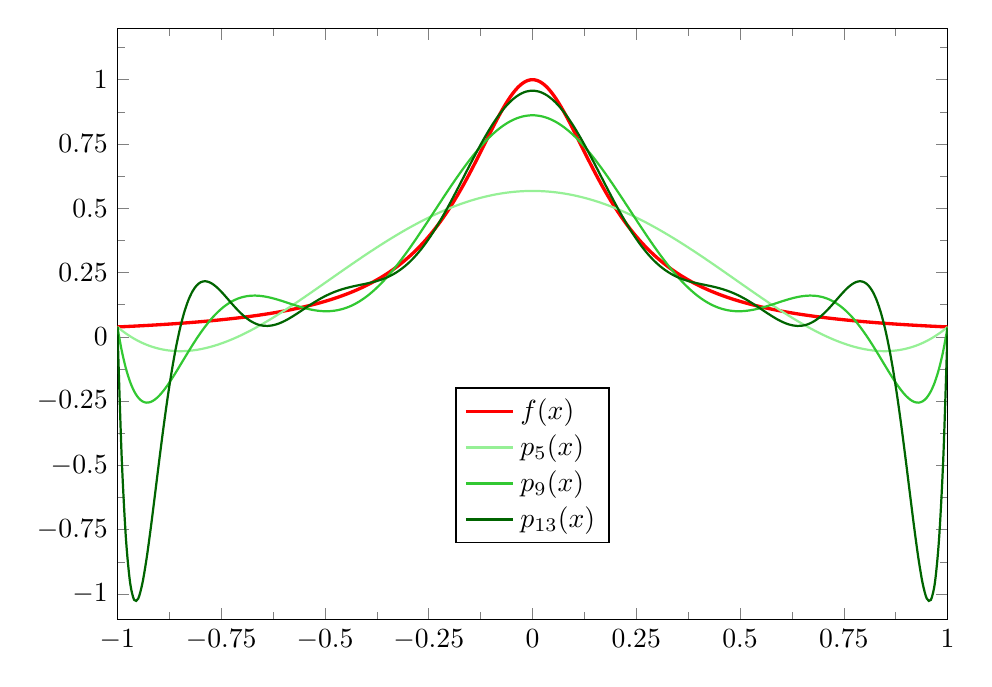
\begin{tikzpicture}
        \begin{axis}[
            xmin = -1, xmax = 1, %
            ymin = -1.1, ymax = 1.2, %
            xtick distance = 0.25, %Is the distance between major ticks in the x-axis.
            ytick distance = 0.25, %Is the distance between major ticks in the y-axis.
            minor tick num = 1, %Is the number of ticks between major ticks.
            major grid style = {lightgray}, %Changes the color and stroke of the major grid.
            minor grid style = {lightgray!25}, %Changes the color and stroke of the minor grid.
            width = \textwidth, %sets the width of the figure
            height = 0.75\textwidth,  %sets the height of the figure
            xlabel = {}, %
            ylabel = {}, %
            legend cell align = {left}, %
            legend style={at={(axis cs:0,-0.5)},anchor=center} % position of the legend box and anchor is the point on the box to be fitted exactly at the point of cs:<>,<>. Options are anchor=center,south west,south east,north west,north east,north,south,west...
        ]
            \addplot[
                domain=-1:1, %Domain of the fucntion
                samples=200, %This parameter determines the number of point to be plotted for the function, while bigger the number better looks the function.
                smooth, %f we use this option, the compiler makes an interpolation between the point plotted to get a soft appearance for the function.
                very thick, %Stroke of the function. Options: ultra thin, very thin, thin, semithick, thick, very thick, ultra thick.
                red %Color of the function.
            ]{1/(1+25*x^2)};
            \addplot[
                domain=-1:1, %Domain of the fucntion
                samples=200, %This parameter determines the number of point to be plotted for the function, while bigger the number better looks the function.
                smooth, %f we use this option, the compiler makes an interpolation between the point plotted to get a soft appearance for the function.
                thick, %Stroke of the function. Options: ultra thin, very thin, thin, semithick, thick, very thick, ultra thick.
                color_green1 %Color of the function.
            ]{1.20192307692308*x^4 - 1.73076923076923*x^2 + 0.567307692307692};
            \addplot[
                domain=-1:1, %Domain of the fucntion
                samples=200, %This parameter determines the number of point to be plotted for the function, while bigger the number better looks the function.
                smooth, %f we use this option, the compiler makes an interpolation between the point plotted to get a soft appearance for the function.
                thick, %Stroke of the function. Options: ultra thin, very thin, thin, semithick, thick, very thick, ultra thick.
                color_green2 %Color of the function
            ]{21.6247747536392*x^8 - 44.9154580808920*x^6 + 30.7285300420963*x^4 - 8.26092332834775*x^2 + 0.861538151965819};
            \addplot[
                domain=-1:1, %Domain of the fucntion
                samples=200, %This parameter determines the number of point to be plotted for the function, while bigger the number better looks the function.
                smooth, %f we use this option, the compiler makes an interpolation between the point plotted to get a soft appearance for the function.
                thick, %Stroke of the function. Options: ultra thin, very thin, thin, semithick, thick, very thick, ultra thick.
                color_green3 %Color of the function
            ]{369.006629567662*x^12 - 5.68434188608080e-14*x^11 - 1008.23965248026*x^10 - 2.16004991671070e-12*x^9 + 1036.16040389924*x^8 - 1.42108547152020e-12*x^7 - 507.215504127014*x^6 + 1.42108547152020e-13*x^5 + 124.636816868829*x^4 - 2.66453525910038e-14*x^3 - 15.2674460668263*x^2 - 8.88178419700125e-16*x + 0.957213876827098};
            \legend{$f(x)$,$p_5(x)$,$p_9(x)$,$p_{13}(x)$}
        \end{axis}
    \end{tikzpicture}
\end{document}